\documentclass[border=4pt]{standalone}
\usepackage{tikz}
\usetikzlibrary{automata, positioning, arrows}
\tikzset{->,  % makes the edges directed
	>=stealth, % makes the arrow heads bold
	node distance=3cm, % specifies the minimum distance between two nodes. Change if necessary.
	every state/.style={thick, fill=blue!10}, % sets the properties for each ’state’ node
%	minimum size=2.5cm,
	initial text=$ $, % sets the text that appears on the start arrow
}
\begin{document}
	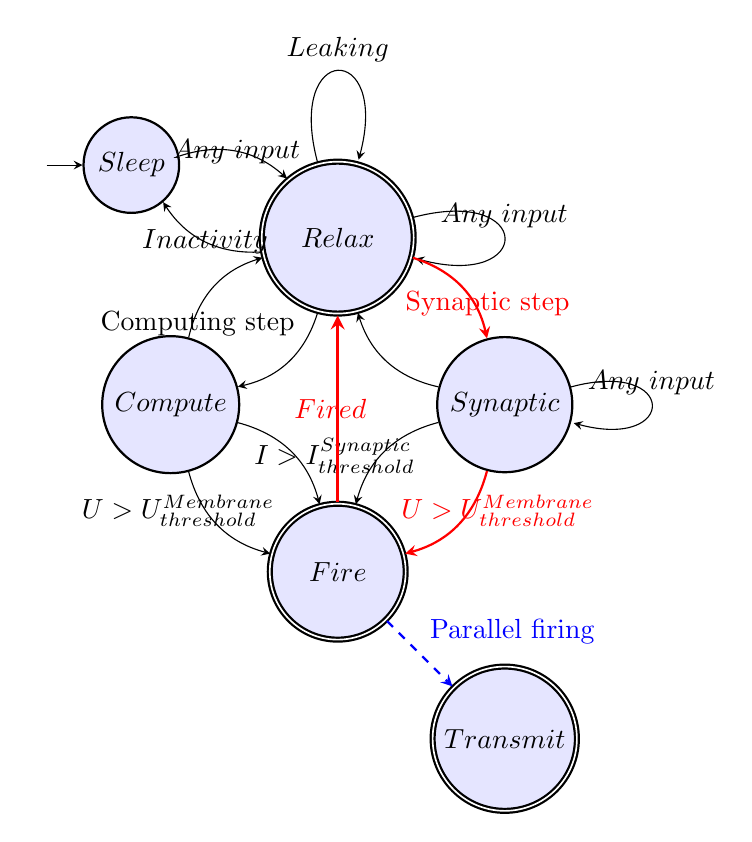
\begin{tikzpicture}
	% Initially, the neurer is ready, but sleeping
	\node[state, initial] (Sleep) {$Sleep$};
	% The major state is 
	\node[state, accepting, below right of=Sleep,yshift=1.2cm,xshift=.5cm] (Acquire) {$\quad Relax\quad$};
	\draw (Sleep) edge[bend left,yshift=.5cm] node{$Any~input$} (Acquire) ;
	\draw (Acquire) edge[bend left] node{$Inactivity$} (Sleep) ;
	\draw   (Acquire) edge[loop right] node[above]{$Any~input$} (Acquire);	
	\draw   (Acquire) edge[loop above] node[above]{$Leaking$} (Acquire);	
	\node[state, below right of=Acquire] (Synaptic) {$Synaptic$};
	\draw   (Synaptic) edge[loop right] node[above]{$Any~input$} (Synaptic);	
	%% Make a synaptic step
	\draw (Acquire) edge[bend left, above left, thick, color=red] node[ xshift=1.5cm,yshift=-.5cm]{Synaptic step} (Synaptic) ;	
	\draw (Synaptic) edge[bend left, above left] node[ xshift=2cm]{ } (Acquire) ;
	%%	Make a computing step, such as PDE solving
	\node[state, below left of=Acquire] (Compute) {$Compute$};
	\draw (Acquire) edge[bend left, above left] node[ xshift=.2cm,yshift=.2cm]{Computing step} (Compute) ;	
	\draw (Compute) edge[bend left, above left] node[ xshift=2cm]{ } (Acquire) ;
	
	%% Will fire, somehow
	\node[state, accepting, below right of=Compute] (Fire) {$\quad Fire\quad$};
	\draw (Compute) edge[bend left, above left] node[ xshift=1.7cm,yshift=-.4cm]{$I>I_{threshold}^{Synaptic}$} (Fire) ;
	\draw (Synaptic) edge[bend right, above left] node[ xshift=1.7cm,yshift=-.2cm]{} (Fire) ;
	%% in steps:
	\node[state, accepting, below right of=Fire] (Firing) {$Transmit$};
	\draw (Fire) edge[above right, thick, dashed,color=blue] node[]{Parallel firing} (Firing) ;	
%\draw (Firing) edge[bend left, above left] node[ xshift=2cm]{ } (Fire) ;
	
	
	\draw (Compute) edge[bend right, below] node[ xshift=-.5cm,
	yshift=.5cm
]{$U>U_{threshold}^{Membrane}$} (Fire) ;

	\draw (Synaptic) edge[bend left, below, thick, color=red] node[ xshift=.5cm,
yshift=.5cm
]{$U>U_{threshold}^{Membrane}$} (Fire) ;
	

%	\node[state, accepting, below left of=Compute] (Relax) {$\ \ Relax \ \ $};
	\draw (Fire) edge[very thick, color=red, left] node[ xshift=.5cm
]{$Fired$} (Acquire) ;
	
%	\draw (Relax) edge[bend left] node[
%yshift=-.5cm
%]{$Relaxed$} (Sleep) ;
%	\node[state, initial] (q1) {$q_1$};
%	\node[state, accepting, right of=q1] (q2) {$q_2$};
%	\node[state, right of=q2] (q3) {$q_3$};
%	\draw   (q1) edge[loop above] node{0} (q1)
%	(q1) edge[above] node{1}
%	(q2)(q2) edge[loop above] node{1} (q2)
%	(q2) edge[bend left, above] node{0} (q3)
%	(q3) edge[bend left, below] node{0, 1} (q2);
	\end{tikzpicture}
\end{document}